\taskpic{Участок цепи постоянного тока состоит из трех одинаковых
  вольтметров и двух одинаковых амперметров. Показания вольтметров
  V$_1$ и V$_2$ равны $U_1 = 6$~B, $U_2 = 4$~B. Как вы полагаете, что
  показывает третий вольтметр?}{
  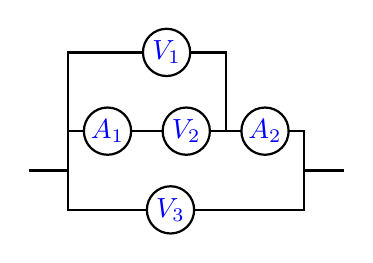
\begin{tikzpicture}
    \draw[thick] (0,0.5) -- (0.5,0.5);
    \draw[thick] (0.5,0.5) -- (0.5,2) -- (1.45,2) (2.05,2) -- (2.5,2) --
    (2.5,1) -- (2.7,1);
    \draw[thick] (1.75,2) circle (0.3cm) node[blue] {$V_1$};
    \draw[thick] (3,1) circle (0.3cm) node[blue] {$A_2$};
    \draw[thick] (3.3,1) -- (3.5,1) -- (3.5,0.5) -- (4,0.5);
    \draw[thick] (0.5,1) -- (0.7,1);
    \draw[thick] (1,1) circle (0.3cm) node[blue] {$A_1$};
    \draw[thick] (2.6,1) -- (2.3,1);
    \draw[thick] (2,1) circle (0.3cm) node[blue] {$V_2$};
    \draw[thick] (1.3,1) -- (1.7,1);
    \draw[thick] (0.5,0.5) -- (0.5,0) -- (1.5,0) (2.1,0) -- (3.5,0) --
    (3.5,1);
    \draw[thick] (1.8,0) circle (0.3cm) node[blue] {$V_3$};
  \end{tikzpicture}
}
% СПб городская олимпиада, районный тур 11 класса, 1992